\documentclass[handout]{beamer}

\usepackage{quantikz}
\usepackage{graphicx}

\title{T-State cultivation : circuit designs}
\author{Dynerowicz S.}
\date{}

\tikzstyle{quantum red}=[red!75!black!50]
\tikzstyle{quantum blue}=[blue!75!black!50]
\tikzstyle{quantum green}=[green!75!black!50]

\tikzstyle{data}=[circle, fill=black, text=white]
\tikzstyle{meas}=[circle, fill=white, draw=black, ultra thick]
\tikzstyle{stabilizer}=[draw=black]

\newcommand{\Op}[1]{{\bf #1}}
\newcommand{\kett}[1]{\ket{\mbox{\tt #1}}}

\begin{document}
	\begin{frame}
		\titlepage
	\end{frame}

	\begin{frame}
		\frametitle{Overview : current design}
		\centering
		\scalebox{0.75}{
			\begin{quantikz}[row sep={between origins, 0.75cm}]
				& \gate[7,style={rounded corners=5pt}][3cm]{\textsc{Injection}}
				& \gate[7,style={rounded corners=5pt}][3cm]{\textsc{Syndrome}}
				& \gate[7,style={rounded corners=5pt, fill=black, inner ysep=-29pt}]{\rotatebox{90}{\color{white}\scshape Post-select}}
				& \gate[7,style={rounded corners=5pt}][3cm]{\textsc{Cultivation}}
				& \\
				&&&&& \\
				&&&&& \\
				&&&&& \\
				&&&&& \\
				&&&&& \\
				&&&&&
			\end{quantikz}
		}
	\end{frame}

	\begin{frame}
		\frametitle{Final configuration for teleportation}
		\begin{itemize}
			\item Superdense code cycle requires $2$ ancillas per plaquette
			\begin{itemize}
				\item n.b. $1$ ancilla for two data qubits in each plaquette
			\end{itemize}
			\item Cultivation requires $6$ ancillas ({\color{red} one shared between $q_{\scriptscriptstyle 1}$ and $q_{\scriptscriptstyle 5}$})
			\begin{itemize}
				\item Could it be shared between $q_{\scriptscriptstyle 1}$ and $q_{\scriptscriptstyle 7}$ instead ?
			\end{itemize}
		\end{itemize}
		\vspace{1cm}
		\centering
		\scalebox{0.65}{
			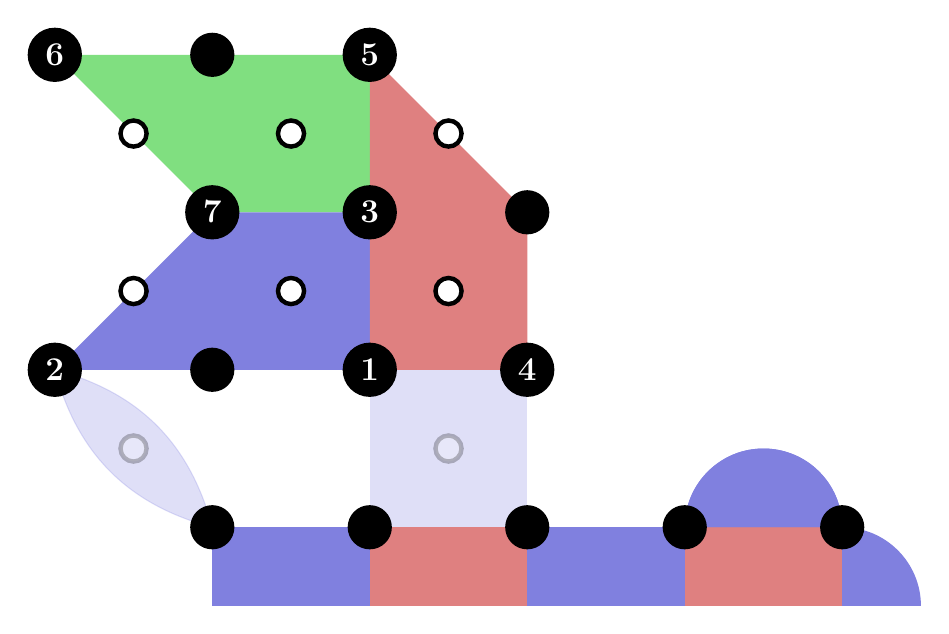
\begin{tikzpicture}
				% Plaquettes of the Steane Code
				\fill[quantum green] (-2, 0) -- ( 2, 0) -- ( 2,-2) -- ( 0,-2);
				\fill[quantum blue]  ( 0,-2) -- (-2,-4) -- ( 2,-4) -- ( 2,-2);
				\fill[quantum red]   ( 2, 0) -- ( 4,-2) -- ( 4,-4) -- ( 2,-4);
	
				% Plaquettes of the Surface Code
				\fill[quantum blue] (0,-6) -- (2, -6) -- (2, -7) -- (0, -7);
				\fill[quantum blue] (4,-6) -- (6, -6) -- (6, -7) -- (4, -7);
				\fill[quantum red] (2,-6) -- (4, -6) -- (4, -7) -- (2, -7);
				\fill[quantum red] (6,-6) -- (8, -6) -- (8, -7) -- (6, -7);
	
				\fill[quantum blue] (6, -6) arc[start angle=180, end angle=0, radius=1.0]
					-- (8, -6) -- cycle;
				\fill[quantum blue] (8, -6) arc[start angle=90, end angle=0, radius=1.0]
					-- (8, -7) -- cycle;
				\fill[quantum blue] (6, -6) arc[start angle=180, end angle=0, radius=1.0]
					-- (8, -6) -- cycle;
	
				\fill[quantum blue, opacity=0.25] (2,-4) -- (4, -4) -- (4, -6) -- (2, -6);
				\filldraw[quantum blue, opacity=0.25] (-2,-4) to[bend left=30] (0,-6) to[bend left=30] (-2,-4);
	
	
				\node[data] at ( 0, 0) {\phantom{o}};
				\node[data] at ( 4,-2) {\phantom{o}};
				\node[data] at ( 0,-4) {\phantom{o}};
	
				\node[data] at ( 2,-4) {\large $\mathbf{1}$};
				\node[data] at (-2,-4) {\large $\mathbf{2}$};
				\node[data] at ( 2,-2) {\large $\mathbf{3}$};
				\node[data] at ( 4,-4) {\large $\mathbf{4}$};
				\node[data] at ( 2, 0) {\large $\mathbf{5}$};
				\node[data] at (-2, 0) {\large $\mathbf{6}$};
				\node[data] at ( 0,-2) {\large $\mathbf{7}$};	
	
				\foreach \x in {-1, 1, 3}{
					\foreach \y in {-3, -1}{
						\node[meas] at (\x,\y) {};
					}
				}
				\foreach \x in {-1, 3}{ \node[meas, opacity=0.25] at (\x,-5) {}; }
	
				\foreach \x in {0, 2, 4, 6, 8}{ \node[data] at (\x, -6) {\phantom{o}}; }
			\end{tikzpicture}
		}	
	\end{frame}


	\begin{frame}
		\frametitle{Final configuration for teleportation}
		\centering
		\begin{itemize}
			\item Superdense code cycle requires $2$ ancillas per plaquette
			\begin{itemize}
				\item[$\hookrightarrow$] Avoid using data qubits for syndrome measurements
			\end{itemize}
		\end{itemize}
		\vspace{1cm}
		\scalebox{0.65}{
			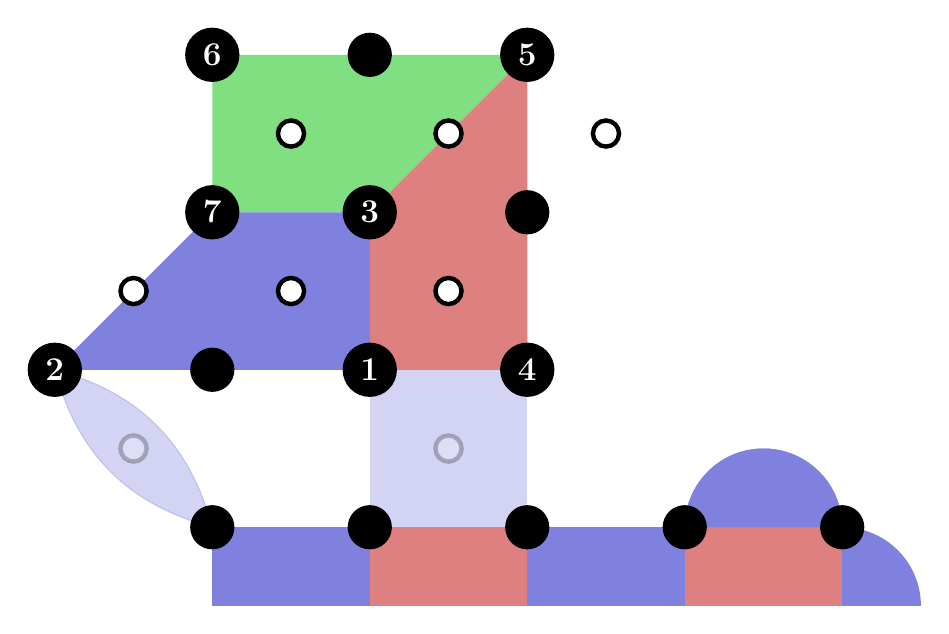
\begin{tikzpicture}
				% Plaquettes of the Steane Code
				\fill[quantum green] (0, 0) -- (4, 0) -- (2,-2) -- (0, -2);
				\fill[quantum blue] (0,-2) -- (-2, -4) -- (2, -4) -- (2, -2);
				\fill[quantum red] (2,-2) -- (2, -4) -- (4, -4) -- (4, 0);
	
				% Plaquettes of the Surface Code
				\fill[quantum blue] (0,-6) -- (2, -6) -- (2, -7) -- (0, -7);
				\fill[quantum blue] (4,-6) -- (6, -6) -- (6, -7) -- (4, -7);
				\fill[quantum red] (2,-6) -- (4, -6) -- (4, -7) -- (2, -7);
				\fill[quantum red] (6,-6) -- (8, -6) -- (8, -7) -- (6, -7);
	
				\fill[quantum blue] (6, -6) arc[start angle=180, end angle=0, radius=1.0]
					-- (8, -6) -- cycle;
				\fill[quantum blue] (8, -6) arc[start angle=90, end angle=0, radius=1.0]
					-- (8, -7) -- cycle;
				\fill[quantum blue] (6, -6) arc[start angle=180, end angle=0, radius=1.0]
					-- (8, -6) -- cycle;
	
				\fill[quantum blue, opacity=0.35] (2,-4) -- (4, -4) -- (4, -6) -- (2, -6);
				\filldraw[quantum blue, opacity=0.35] (-2,-4) to[bend left=30] (0,-6) to[bend left=30] (-2,-4);
	
	
				\node[data] at (2, 0) {\phantom{o}};
				\node[data] at (4,-2) {\phantom{o}};
				\node[data] at (0,-4) {\phantom{o}};
	
				\node[data] at (2,-4) {\large $\mathbf{1}$};
				\node[data] at (-2,-4) {\large $\mathbf{2}$};
				\node[data] at (2,-2) {\large $\mathbf{3}$};
				\node[data] at (4,-4) {\large $\mathbf{4}$};
				\node[data] at (4, 0) {\large $\mathbf{5}$};
				\node[data] at (0, 0) {\large $\mathbf{6}$};
				\node[data] at (0,-2) {\large $\mathbf{7}$};	
	
				\foreach \x in {1, 3, 5}{ \node[meas] at (\x,-1) {}; }
				\foreach \x in {-1, 1, 3}{ \node[meas] at (\x,-3) {}; }
				\foreach \x in {-1, 3}{ \node[meas, opacity=0.25] at (\x,-5) {}; }
	
				\foreach \x in {0, 2, 4, 6, 8}{ \node[data] at (\x, -6) {\phantom{o}}; }
			\end{tikzpicture}
		}

	\end{frame}

	\begin{frame}
		\frametitle{\sc Injection --- Abstract circuit}
		\begin{itemize}
			\item Preparation of a Steane Code logical T-state on $7$ qubits
			\begin{equation*}
				\ket{\Op{T}}_{\scriptscriptstyle L} ~=~ \kett{0}_{\scriptscriptstyle L} + e^{i\pi/4}\kett{1}_{\scriptscriptstyle L}	
			\end{equation*}
		\end{itemize}
		\vspace{0.5cm}
		\begin{minipage}{0.32\textwidth}
			\centering
			\scalebox{0.6}{
				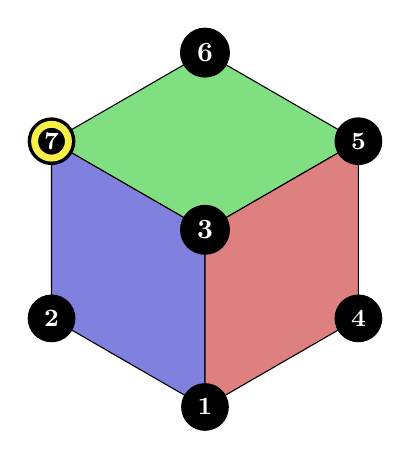
\begin{tikzpicture}
					\coordinate (O) at (0,0);
					\coordinate (A) at ( 30:2.25);
					\coordinate (B) at ( 90:2.25);
					\coordinate (C) at (150:2.25);
					\coordinate (D) at (210:2.25);
					\coordinate (E) at (270:2.25);
					\coordinate (F) at (330:2.25);
	
					\fill[quantum green, stabilizer] (O) -- (A) -- (B) -- (C) -- cycle;
					\fill[quantum blue, stabilizer]  (O) -- (C) -- (D) -- (E) -- cycle;
					\fill[quantum red, stabilizer]  (O) -- (E) -- (F) -- (A) -- cycle;
	
					\node[data] at (E) {\small $\mathbf{1}$};
					\node[data] at (D) {\small $\mathbf{2}$};
					\node[data] at (O) {$\mathbf{3}$};
					\node[data] at (F) {\small $\mathbf{4}$};
					\node[data] at (A) {\small $\mathbf{5}$};
					\node[data] at (B) {$\mathbf{6}$};
					\node[data] at (C) {\small $\mathbf{7}$};
					\node[circle, draw=yellow!95!black!75, line width=2.5pt] at (C) {\phantom{.}};
				\end{tikzpicture}
			}
		\end{minipage}
		\begin{minipage}{0.62\textwidth}
			\centering
			\scalebox{0.6}{
				\begin{quantikz}[row sep=0.6cm]
					\lstick{$q_{\scriptscriptstyle 1}$}\wireoverride{n} & \midstick{$\kett{+}$~}\wireoverride{n}
					& \ctrl{1} && \ctrl{3}  && \slice{} &&&&&&
					\rstick[7]{~~$\ket{\Op{T}}_{\scriptscriptstyle L}$}
					\\
					\lstick{$q_{\scriptscriptstyle 2}$}\wireoverride{n} & \midstick{$\kett{0}$~}\wireoverride{n}
					& \targ{}  & \targ{}   &\phantom{i}& \targ{}   &
					&          & \ctrl{5}  && \ctrl{5}  &&
					\\
					\lstick{$q_{\scriptscriptstyle 3}$}\wireoverride{n} & \midstick{$\kett{+}$~}\wireoverride{n}
					& \ctrl{1} & \ctrl{-1} &\phantom{i}&\phantom{i}& \ctrl{3} &&\phantom{i}&&\phantom{i}&&
					\\
					\lstick{$q_{\scriptscriptstyle 4}$}\wireoverride{n} & \midstick{$\kett{0}$~}\wireoverride{n}
					& \targ{}  & \targ{} & \targ{}   &\phantom{i}&\phantom{i}
					&&\phantom{i}&&\phantom{i}&&
					\\
					\lstick{$q_{\scriptscriptstyle 5}$}\wireoverride{n} & \midstick{$\kett{+}$~}\wireoverride{n}
					& \ctrl{1} & \ctrl{-1} &&\phantom{i}&\phantom{i}&&\phantom{i}&&\phantom{i}&&
					\\
					\lstick{$q_{\scriptscriptstyle 6}$}\wireoverride{n} & \midstick{$\kett{0}$~}\wireoverride{n}
					& \targ{} & \targ{} &&\phantom{i}& \targ{} & \ctrl{1} &\phantom{i}&&\phantom{i}& \ctrl{1} &
					\\[-0.2cm]
					\lstick{$q_{\scriptscriptstyle 7}$}\wireoverride{n} & \midstick{$\kett{+}$~}\wireoverride{n}
					&& \ctrl{-1} && \ctrl{-5} && \targ{} & \targ{} & \gate[style={fill=yellow!95!black!75}]{\Op{T}^{\dagger}} & \targ{} & \targ{} &
				\end{quantikz}
			}
		\end{minipage}
	\end{frame}

	\begin{frame}
		\frametitle{\textsc{Injection} --- Actual circuit}
		\begin{itemize}
			\item Preparation of $\ket{\Op{T}}_{\scriptscriptstyle L}$: $13$ CNOTs
			\item[$\hookrightarrow$] Move qubits to suitable locations: $18$ CNOTs
			\item Total depth: $12$
		\end{itemize}
		\vspace{1cm}
		\begin{minipage}{0.45\textwidth}
			\centering
			\scalebox{0.5}{
				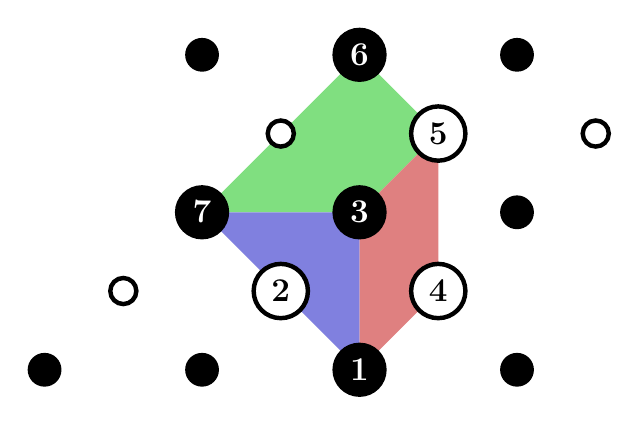
\begin{tikzpicture}
					% Plaquettes of the Steane Code
					\fill[quantum green] (2, 0) -- (3,-1) -- (2,-2) -- (0, -2);
					\fill[quantum blue] (0,-2) -- (2, -4) -- (2, -2);
					\fill[quantum red] (2,-2) -- (3, -1) -- (3, -3) -- (2,-4);

					\node[data] at ( 2, 0) {\phantom{.}};
					\node[data] at ( 4,-2) {\phantom{.}};
					\node[data] at ( 0,-4) {\phantom{.}};
					\node[data] at (-2,-4) {\phantom{.}};

					\node[data] at (2,-4) {\large $\mathbf{1}$};
					\node[meas] at (1,-3) {\large $\mathbf{2}$};
					\node[data] at (2,-2) {\large $\mathbf{3}$};
					\node[meas] at (3,-3) {\large $\mathbf{4}$};
					\node[meas] at (3,-1) {\large $\mathbf{5}$};
					\node[data] at (2, 0) {\large $\mathbf{6}$};
					\node[data] at (0,-2) {\large $\mathbf{7}$};	

					\node[data] at ( 0, 0) {\phantom{.}};
					\node[data] at ( 4, 0) {\phantom{.}};
					\node[data] at ( 4,-4) {\phantom{.}};

					\foreach \x in {1, 5}{ \node[meas] at (\x,-1) {}; }
					\node[meas] at (-1,-3) {};
				\end{tikzpicture}
			}
		\end{minipage}
		$\rightarrow$
		\begin{minipage}{0.45\textwidth}
			\centering
			\scalebox{0.5}{
				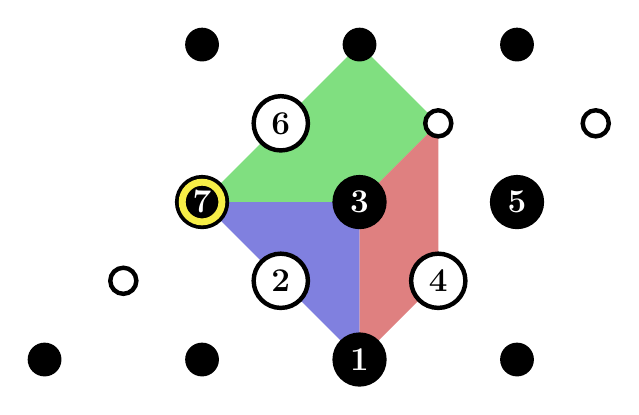
\begin{tikzpicture}
					% Plaquettes of the Steane Code
					\fill[quantum green] (2, 0) -- (3,-1) -- (2,-2) -- (0, -2);
					\fill[quantum blue] (0,-2) -- (2, -4) -- (2, -2);
					\fill[quantum red] (2,-2) -- (3, -1) -- (3, -3) -- (2,-4);

					\node[data] at ( 2, 0) {\phantom{.}};
					\node[data] at ( 4,-2) {\phantom{.}};
					\node[data] at ( 0,-4) {\phantom{.}};
					\node[data] at (-2,-4) {\phantom{.}};

					\node[data] at (2,-4) {\large $\mathbf{1}$};
					\node[meas] at (1,-3) {\large $\mathbf{2}$};
					\node[data] at (2,-2) {\large $\mathbf{3}$};
					\node[meas] at (3,-3) {\large $\mathbf{4}$};
					\node[data] at (4,-2) {\large $\mathbf{5}$};
					\node[meas] at (1,-1) {\large $\mathbf{6}$};
					\node[data] at (0,-2) {\large $\mathbf{7}$};	
					\node[circle, draw=yellow!95!black!75, line width=2.5pt] at (0,-2) {\scalebox{0.75}{\phantom{o}}};

					\node[data] at ( 0, 0) {\phantom{.}};
					\node[data] at ( 4, 0) {\phantom{.}};
					\node[data] at ( 4,-4) {\phantom{.}};

					\foreach \x in {3, 5}{ \node[meas] at (\x,-1) {}; }
					\node[meas] at (-1,-3) {};
				\end{tikzpicture}
			}
%			\scalebox{0.5}{
%				\begin{tikzpicture}
%					% Plaquettes of the Steane Code
%					\fill[quantum green] (0, 0) -- (4, 0) -- (2,-2) -- (0, -2);
%					\fill[quantum blue] (0,-2) -- (-2, -4) -- (2, -4) -- (2, -2);
%					\fill[quantum red] (2,-2) -- (2, -4) -- (4, -4) -- (4, 0);
%
%					\node[data] at (2, 0) {\phantom{o}};
%					\node[data] at (4,-2) {\phantom{o}};
%					\node[data] at (0,-4) {\phantom{o}};
%
%					\node[data] at ( 2,-4) {\large $\mathbf{1}$};
%					\node[data] at (-2,-4) {\large $\mathbf{2}$};
%					\node[data] at ( 2,-2) {\large $\mathbf{3}$};
%					\node[data] at ( 4,-4) {\large $\mathbf{4}$};
%					\node[data] at ( 4, 0) {\large $\mathbf{5}$};
%					\node[data] at ( 0, 0) {\large $\mathbf{6}$};
%					\node[data] at ( 0,-2) {\large $\mathbf{7}$};	
%
%					\foreach \x in {1, 3, 5}{ \node[meas] at (\x,-1) {}; }
%					\foreach \x in {-1, 1, 3}{ \node[meas] at (\x,-3) {}; }
%				\end{tikzpicture}
%			}
		\end{minipage}
	\end{frame}

	\begin{frame}
		\frametitle{\sc Syndrome}
		
	\end{frame}

	\begin{frame}
		\frametitle{\sc Cultivation}
		\centering
		\vspace{0.5cm}
		\scalebox{0.75}{
			\begin{quantikz}[row sep={0.85cm, between origins}, column sep={0.3cm}]
				% Data qubit 6
				\lstick{$q_{6}$} & \gate{\Op{T}^\dagger} && \targ{} &&&&
				& &&&&\targ{} && \gate{\Op{T}} & \\
				% Ancilla 1
				&\wireoverride{n}& \midstick{$\kett{+}$}\wireoverride{n} & \ctrl{-1} & \targ{} &&&
				& &&&\targ{}&\ctrl{-1} & \meter{\scalebox{0.5}{\Op{X}}}\\
				% Data qubit 7
				\lstick{$q_{7}$} & \gate{\Op{T}^\dagger} & &\targ{} & \ctrl{-1} &\targ{}&&
				& &&\targ{}&\ctrl{-1}&\targ{}&&\gate{\Op{T}} & \\
				% Ancilla 2
				&\wireoverride{n}& \midstick{$\kett{+}$}\wireoverride{n} & \ctrl{-1} &&\phantom{i}&&
				& &&\phantom{i}&&\ctrl{-1}& \meter{\scalebox{0.5}{\Op{X}}}\\
				% Data qubit 2
				\lstick{$q_{2}$} & \gate{\Op{T}^\dagger} & &\targ{} &&\phantom{i}&&
				& &&\phantom{i}&&\targ{}&&\gate{\Op{T}} &\\
				% Ancilla 3
				&\wireoverride{n}& \midstick{$\kett{+}$}\wireoverride{n} & \ctrl{-1} &\targ{}&\phantom{i}&&
				& &&\phantom{i}&\targ{}&\ctrl{-1}& \meter{\scalebox{0.5}{\Op{X}}}\\
				% Data qubit 3
				\lstick{$q_{3}$} & \gate{\Op{T}^\dagger} & &\targ{} &\ctrl{-1}&\ctrl{-4}&\ctrl{3}& \meter{\scalebox{0.5}{\Op{X}}}
				& \wireoverride{}\midstick{$\kett{+}$} &\ctrl{3}&\ctrl{-4}&\ctrl{-1}&\targ{}&& \gate{\Op{T}} &\\
				% Ancilla 4
				&\wireoverride{n}& \midstick{$\kett{+}$}\wireoverride{n} & \ctrl{-1} &&&\phantom{i}&
				& &\phantom{i}&&&\ctrl{-1}& \meter{\scalebox{0.5}{\Op{X}}}\\
				% Data qubit 1
				\lstick{$q_{1}$} & \gate{\Op{T}^\dagger} & &&&\targ{}&\phantom{i}&
				& &\phantom{i}&\targ{}&&&&\gate{\Op{T}} & \\
				% Ancilla 5
				&\wireoverride{n}& \midstick{$\kett{+}$}\wireoverride{n} & \ctrl{1} &\ctrl{2}&\ctrl{-1}&\targ{}&
				& &\targ{}&\ctrl{-1}&\ctrl{2}&\ctrl{1}& \meter{\scalebox{0.5}{\Op{X}}}\\
				% Data qubit 5
				\lstick{$q_{5}$} & \gate{\Op{T}^\dagger} & &\targ{} &\phantom{i}&&&
				& &&&\phantom{i}&\targ{}&&\gate{\Op{T}} & \\
				% Ancilla 6
				&\wireoverride{n}& \midstick{$\kett{+}$}\wireoverride{n} & \ctrl{1} &\targ{}&&&
				& &&&\targ{}&\ctrl{1}& \meter{\scalebox{0.5}{\Op{X}}}\\
				% Data qubit 4
				\lstick{$q_{4}$} & \gate{\Op{T}^\dagger} & &\targ{} &&&&
				& &&&&\targ{}&&\gate{\Op{T}} & \\
			\end{quantikz}
		}
	\end{frame}

\end{document}